\documentclass[a4paper, 11pt]{article}

%%% Zeichenkodierung, Rechtschreibung und Umlaute
\usepackage[utf8]{inputenc}
\usepackage[ngerman]{babel}
\usepackage[T1]{fontenc}

%%% Mathematische Symbole, Gleichungen
\usepackage[fleqn]{amsmath}
\usepackage{amsfonts}
\usepackage{amssymb}
\usepackage{amsthm}
\usepackage{mathtools}
\usepackage{bm}
%\usepackage{colonequals} % Zusätzliche Relationssymbole

%%% Tabellen
\usepackage{tabularx}
\usepackage{array}
\usepackage{multicol}

%%% Seitenformat und -ränder
%%% -Alternative 1-
\usepackage{geometry}
\geometry{a4paper, top=25mm, bottom=20mm, left=20mm, right=20mm}
%%% -Alternative 2-
%\usepackage[headheight=110pt]{geometry}
%\geometry{a4paper,left=30mm,right=30mm, top=35mm, bottom=30mm}

%%% Seitenstile (Kopf- und Fußzeile)
\usepackage{fancyhdr}
\pagestyle{fancy}

%%% Sonstiges
\usepackage{caption} % Untertitel von Grafiken/Tabellen manipulieren
\usepackage{enumerate} % Aufzählungszeichen ändern
\usepackage{graphicx} % Standarderweiterung für Bilddateien
\usepackage{hyperref} % Hyperlinks
\usepackage{lastpage} % Berechnung der Seitenzahl
%\usepackage{polynom} % Polynomdivision
\usepackage{setspace} % Zeilenabstand
%\usepackage{textgreek} % griechische Symbole
\usepackage{tikz} % Umfassendes Tool, um Grafiken zu erstellen
\usepackage{verbatim} % Schreibmaschinen-Stil (für Code-Ausschnitte)
\usepackage{float}

%%% Eingaben (z.B. für das Deckblatt)
\newcommand{\module}{Embedded System Design -- Protokoll}
\newcommand{\semester}{Sommersemester 2018}
\newcommand{\finishingdate}{29.06.2018}
\newcommand{\titletext}{Video  Audio Streaming} %TODO: Nummer anpassen

%%%-- Für das Deckblatt --
\title{
	~\\[4cm]
	\textbf{
		\module\\[0.25cm]
		\normalsize \semester \\[1.5cm]
		\Huge\titletext\\
	}
}

\author{
  \vspace{3.5cm}\\
  \begin{tabular}{l}
    \textbf{Gruppe 15:}\\\hline
    Omid Rahimian Mashhadi \\
    Torsten Michael Schenk\\
  \end{tabular}
}

\date{
	\vfill
	Abgabedatum: \finishingdate\\
	\vspace{5mm}
	Seitenanzahl: \pageref{LastPage}
}

%%% -- Kopf- und Fußzeile --
%%% Kopfzeile linker Bereich
\lhead[\leftmark]{\textbf{\module}}
%%% Kopfzeile mittlerer Bereich
\chead[\rightmark]{\rightmark{\titletext}}
%%% Kopfzeile linker Bereich
\rhead{\textbf{zum \finishingdate}}
%%% Fußzeile
\cfoot{\thepage  \ / \pageref{LastPage}}

%%% Serifenfreie Fonts benutzen
%\renewcommand{\familydefault}{\sfdefault}

%%% Font
\usepackage{charter}

%%% Tiefe der Einrückung nach Absätzen
\setlength{\parindent}{0pt}

%%% Evtl. Änderungen des Typs einer Aufzählungsebene (z.B. zur Anpassung an das Aufgabenblatt)
%\renewcommand{\labelenumi}{\alph{enumi})}
%\renewcommand{\labelenumii}{(\roman{enumii})}
%\renewcommand{\labelenumiii}{\arabic{enumiii}.}
%\renewcommand{\labelenumii}{\textbf{-}}

\begin{document}

%%% Deckblatt
\maketitle
\thispagestyle{empty} % Keine Seitenzahl hier
\newpage

%%% Seitenzahl zurücksetzen
\clearpage
\setcounter{page}{1}

%%% Zeilenabstand
%\singlespacing
\onehalfspacing
%\doublespacing

%%%-- Eigentlicher Inhalt --
\section{Projektbeschreibung}

Beschreibung des Projektes...


\begin{minipage}{\textwidth}
    \begin{center}
        Caption for image
        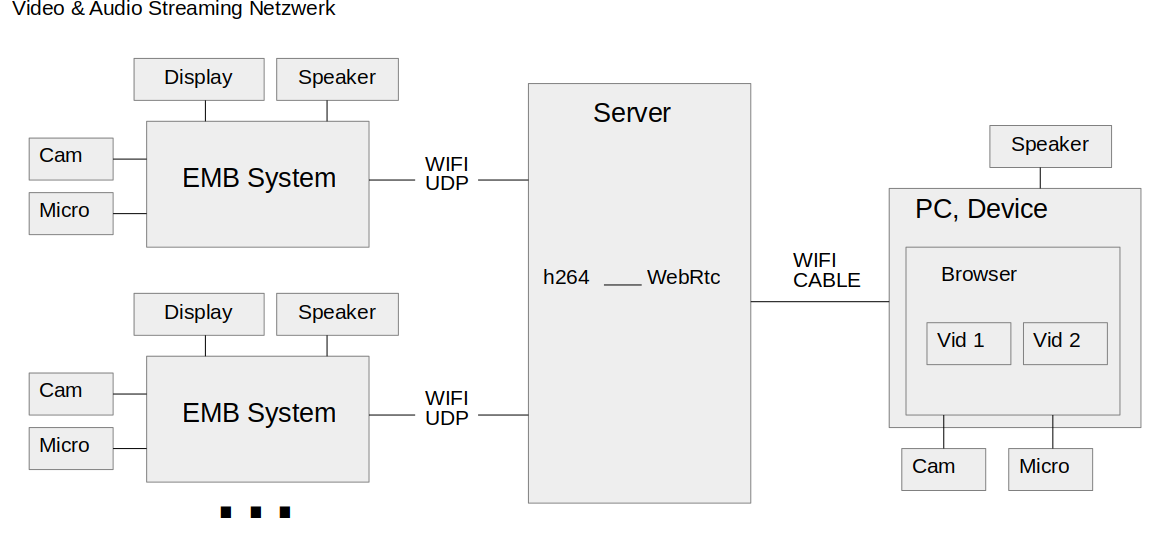
\includegraphics[scale=0.4]{img/schemaproj.png} 
    \end{center}
\end{minipage}


Beschreibung der Schritte zum erreichen des Projektes
...

\section{ffmpeg, ffserver, ffplay}

\textbf{Linux / Raspian ffmpeg} %and pi\_jessie\_motion}

\begin{enumerate}
	\item remove (still needed?):\\
	sudo apt-get remove libavcodec-extra-56 libavformat56 libavresample2 libavutil54
	\item download ffmpeg precompiled armhf.deb:\\
	wget https://github.com/ccrisan/motioneye/wiki/precompiled/ffmpeg\_3.1.1-1\_armhf.deb\\
	sudo dpkg -i ffmpeg\_3.1.1-1\_armhf.deb
	%\item install:\\
	%sudo apt-get install curl libssl-dev libcurl4-openssl-dev libjpeg-dev libx264-142     
	%libavcodec56 libavformat56 libmysqlclient18 libswscale3 libpq5
	%\item install motion:\\
	%wget https://github.com/Motion-Project/motion/releases/download/release-4.0.1/pi\_jessie\_motion\_4.0.1-1\_armhf.deb\\
	%sudo dpkg -i pi\_jessie\_motion\_4.0.1-1\_armhf.deb
\end{enumerate}


\section{Motion Installation \& Test}

Motion ist ein Programm, das in der Lage ist zu erkennen, wenn ein signifikanter Teil des Kamerabildes sich verändert. Es kann also 
Bewegung erkennen und einen Warnton übertragen. Kamera streaming 
Service welches verwendet werden kann, um den Videostream 
einer Webcam an eine IP Adresse zu leiten. Motion kann mit 
vielen Geräten verwendet werden. Unterstützt werden:
\begin{itemize}
\item V4L2 Webcams (closed source)
\item Video Frame Grabber
\item Network Kameras via HTTP, RTSP, RTMP
\item PI Kameramodul
\item Webcam
\end{itemize}

Video Stream zur IP Adresse des Devices (Raspi) im es im lokalen 
Netzwerk um Browser anzuzeigen....TODO

OP: Raspian\\
Setup: Streaming server motion\\

Anleitung nach Tutorial mit Anpassungen:\\
https://pimylifeup.com/raspberry-pi-webcam-server/\\

\textbf{Jessie and Strech are two debian major release}\\
Debian 9 (stretch) — current stable release\\
Debian 8 (jessie) — obsolete stable release\\

\textbf{Raspian pi\_streach\_motion}

\begin{enumerate}
	\item install:\\
	sudo apt-get install libmariadbclient18 libpq5 libavcodec57  libavformat57 libavutil55 libswscale4\\
	einige Pakete sind outdated und müssen durch aktuelle ersetzt werden:\\
	sudo apt install libx264-148\\
	libavcodec57\\
	libavformat57\\
	libmariadbclient-dev-compat\\
	default-libmysqlclient-dev\\
	libswscale

	\item download motion stretch deb\\
	sudo wget https://github.com/Motion-Project/motion/releases/download/release-4.0.1/pi\_stretch\_motion\_4.0.1-1\_armhf.deb\\
	sudo dpkg -i pi\_stretch\_motion\_4.0.1-1\_armhf.deb\\

	Configuring Motion:\\
	sudo vim /etc/motion/motion.conf\\
	daemon on\\
	stream\_localhost off\\
	if problems with freezing if motion occures\\
	output\_pictures off\\
	ffmpeg\_output\_movies off\\
	optional\\
	stream\_maxrate 100\\
	framerate 100\\
	width 640\\
	height 480

	\item setup daemon\\
	sudo vim /etc/default/motion\\
	start\_motion\_daemon=yes
\end{enumerate}

start stop motion and streaming by:\\
sudo service motion start\\
sudo service motion stop\\

check browser in local network, xxx ip adress of raspi (ip addr show):\\
192.168.1.xxx:8081

How to test if video and avi works at all:\\
Test raspi video codex and sound from avi video\\
omxplayer -p -o local dolbycanyon.avi\\
-o local = headphone jack

\section{Audio}
Um Audio auf den Headphone Jack umzuleiten (default ist HDMI) zuerst pulseaudio deinstallieren.\\
sudo apt remove pulseaudio\\

Dann die richtige Zuordnung setzen, 1 steht für local audio jack:\\
amixer cset numid=3 1
amixer cset numid=2 1\\
oder \\
amixer -c 0 cset numid=3 1\\

Audio Tests:\\
aplay /usr/share/scratch/Media/Sounds/Vocals/Singer1.wav\\
Facebook Video Call: OK (schlechter Sound)\\
Musikvidoes auf YoutTube: OK (guter Sound)\\

\section{h264}

Beschreibung des Projektes...


\begin{minipage}{\textwidth}
    \begin{center}
        Caption for image
        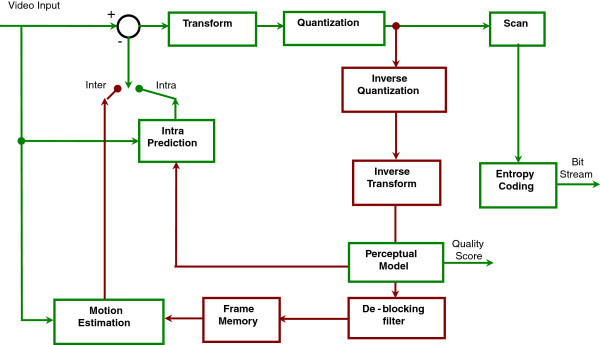
\includegraphics[scale=4.0]{img/h264.jpg} 
    \end{center}
\end{minipage}



\section{gstreamer}

Wenn Fehler beim Compilieren eines gstream Testprogramms auftreten, z.B.
\begin{verbatim}
Package gstreamer-1.0 was not found in the pkg-config search path.
Perhaps you should add the directory containing `gstreamer-1.0.pc'
to the PKG_CONFIG_PATH environment variable
No package 'gstreamer-1.0' found
playback-tutorial-6.c:1:10: fatal error: gst/gst.h: No such file or directory
\end{verbatim}

gstreamer-1.0 ist der folgenden lib enthalten:\\
sudo apt install libgstreamer1.0-dev\\

\textbf{Beispiel Programme gstreamer kompilieren}
gcc playback-tutorial-6.c -o playback-tutorial-6 `pkg-config --cflags --libs gstreamer-1.0`

\section{Strato Web Server}

\textbf{Login via ssh}\\
ssh -X root@85.214.211.169\\
ssh -X root@85.214.211.169 -L 5901:localhost:5901\\
pwd: xxxxxxxxxx (pwd vom Provider)

\textbf{Remote Desktop}\\
tightvncserver: server\\
xtightvncviewer: viewer\\
sudo apt install tightvncserver xtightvncviewer\\
\# set xtightvnciewer pwd\\

\textbf{Full Login}\\
ssh -X root@85.214.211.169 -L 5901:localhost:5901\\
ssh Passwort eingeben\\
\# Start vncserver\\
vncserver :1\\
echo \grqq{}\$DISPLAY\grqq{}\\
\# in server ssh console\\
xtightvncviewer 127.0.0.1:1\\
vnc Passwort eingeben\\
\# X Fenster sollte sich öffnen








\newpage
\section{Rapsi Touchscreen Display}

\# Zeige Namen aller angeschlossenen Displays\\
xrandr -q\\

\# 180 Grad drehen\\
xrandr --output HDMI-1 --rotate inverted\\

\# Touchscreen muss auch rotiert werden\\
\# bitte einfügen in /boot/config.txt:\\
\# rote touchscreen (display rotated via xrandr startup script)\\
lcd\_rotate=2\\



\section{noch eins}

\section*{Definitionen Fachbegriffe:}

Test

\end{document}
